\documentclass[tikz,border=5pt]{standalone}
\usetikzlibrary{positioning,arrows.meta}

\begin{document}

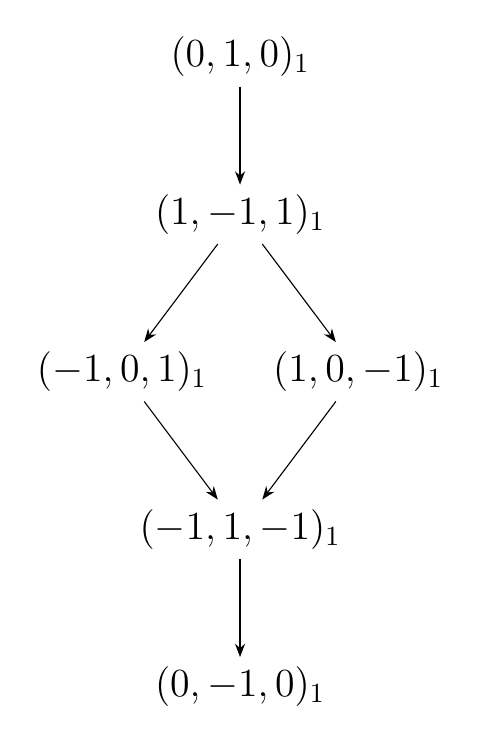
\begin{tikzpicture}[
    >=Stealth,
    every node/.style={font=\Large},
    node distance=2.3cm
]

\node (a) at (1.5,0) {$(0, 1, 0)_1$};

\node (b) at (1.5,-2.0) {$(1, -1, 1)_1$};

\node (c1) at (0,-4.0) {$(-1, 0, 1)_1$};
\node (c2) at (3,-4.0) {$(1, 0, -1)_1$};

\node (d) at (1.5,-6.0) {$(-1, 1, -1)_1$};

\node (e) at (1.5,-8.0) {$(0, -1, 0)_1$};

\draw[->] (a) -- (b);

\draw[->] (b) -- (c1);
\draw[->] (b) -- (c2);

\draw[->] (c1) -- (d);
\draw[->] (c2) -- (d);

\draw[->] (d) -- (e);

\end{tikzpicture}

\end{document}